% report/ExpCmain000.tex
\documentclass[18pt,c]{beamer}
\makeatletter
\let\beamer@writeslidentry@miniframeson=\beamer@writeslidentry
\def\beamer@writeslidentry@miniframesoff{%
  \expandafter\beamer@ifempty\expandafter{\beamer@framestartpage}{}% does not happen normally
  {%else
    % removed \addtocontents commands
   \clearpage\beamer@notesactions%
  }
}
\newcommand*{\miniframeson}{\let\beamer@writeslidentry=\beamer@writeslidentry@miniframeson}
\newcommand*{\miniframesoff}{\let\beamer@writeslidentry=\beamer@writeslidentry@miniframesoff}
\makeatother
% yellow
\definecolor{goldenyellow}{rgb}{1.0, 0.87, 0.0}
\definecolor{electricyellow}{rgb}{1.0, 1.0, 0.0}
\definecolor{icterine}{rgb}{0.99, 0.97, 0.37}
\definecolor{flavescent}{rgb}{0.97, 0.91, 0.56}
\definecolor{lemon}{rgb}{1.0, 0.97, 0.0}
% orange
\definecolor{amber}{rgb}{1.0, 0.75, 0.0}
\definecolor{cadmiumorange}{rgb}{0.93, 0.53, 0.18}
\definecolor{internationalorange}{rgb}{1.0, 0.31, 0.0}
% red
\definecolor{ferrarired}{rgb}{1.0, 0.11, 0.0}
\definecolor{fireenginered}{rgb}{0.81, 0.09, 0.13}
\definecolor{cadmiumred}{rgb}{0.89, 0.0, 0.13}
% blue
\definecolor{ao}{rgb}{0.0, 0.5, 0.0}
\definecolor{babyblueeyes}{rgb}{0.63, 0.79, 0.95}
\definecolor{bleudefrance}{rgb}{0.19, 0.55, 0.91}
\definecolor{blue}{rgb}{0.0, 0.0, 1.0}
\definecolor{cobalt}{rgb}{0.0, 0.28, 0.67}
\definecolor{darkmidnightblue}{rgb}{0.0, 0.2, 0.4}
\definecolor{brandeisblue}{rgb}{0.0, 0.44, 1.0}
\definecolor{deepskyblue}{rgb}{0.0, 0.75, 1.0}
\definecolor{iris}{rgb}{0.35, 0.31, 0.81}
\definecolor{navyblue}{rgb}{0.0, 0.0, 0.5}
\definecolor{ultramarine}{rgb}{0.07, 0.04, 0.56}
\definecolor{electricultramarine}{rgb}{0.25, 0.0, 1.0}
% green
\definecolor{cadmiumgreen}{rgb}{0.0, 0.42, 0.24}
\definecolor{darkpastelgreen}{rgb}{0.01, 0.75, 0.24}
\usetheme{Berlin}
\usecolortheme{default}
\usefonttheme{default}
\setbeamerfont{frametitle}{size=\footnotesize}
\usepackage{graphicx}
\renewcommand{\topfraction}{1.0}
\renewcommand{\floatpagefraction}{1.0}
\begin{document}
\title{Report of Experiment ExpC. 3-Symmetry: Replay. }
\author{Andreas Geyer-Schulz}
\date{\today}
\begin{frame}
\titlepage
\end{frame}
\begin{frame}
\frametitle{Abstract}
This experiment tests exact replication and stochastic replication
for {\tt xegaRun} of R-package {\tt xega}.
In the experiment, the 3-symmetry problem is solved
by grammar-based genetic programming for fixed seeding and for
Rs system seeding (option {\tt replay} of {\tt xegaRun}).%\end{abstract}
\end{frame}
\begin{frame}[t, allowframebreaks]
\frametitle{Contents}
\tableofcontents[subsubsectionstyle=hide]
\vfill
\end{frame}
% report/ExpCmain001.tex
\miniframeson
\section{Design of Experiment}
% report/ExpCmain002.tex
\begin{frame}
\vspace*{2mm}
\begin{block}{
Definitions
}
{\bf Exact replicability} of a computational experiment means
that the experiment procudes in each trial {\bf identical}
numerical result.
 
{\bf Stochastic replicability} of a computational experiment means
that the experiment procudes in each trial the same 
expected result.
\end{block}
\end{frame}% report/ExpCmain003.tex
\begin{frame}
\vspace*{2mm}
\begin{block}{
Description of Experiment
}
The purpose of this computational experiment is to show the difference
between {\bf exact} and {\bf stochastic} replicability of the experiment.
 
The {\bf problem environment} is the 3-symmetry problem: 
Finding a boolean expression (with and, or, and not)
which is TRUE for symmetric 3-bit strings.
 
The {\bf solution method} is grammar-based genetic programming
(option {\tt algorithm="sgp"}  of {\tt xegaRun}).
The {\bf solver} used is {\tt xegaRun} from the R-package {\tt xega}.
 
The experiment consists of 4 treatments, two for each choice of seeding.
\end{block}
\end{frame}% report/ExpCmain004.tex
% ExpC
% Table: Common Parameters of Experiment ExpC
% Sun May 11 22:53:05 2025
 \begin{frame}
 \fontsize{8pt}{9pt}\selectfont
 \frametitle{ Common Parameters of Experiment ExpC }
% latex table generated in R 4.4.3 by xtable 1.8-4 package
% Sun May 11 22:53:05 2025
\begin{table}[ht]
\centering
\begin{tabular}{rr}
  \hline
 & Parameter Value \\ 
  \hline
Experiment & ExpC \\ 
  Problem.Environment & 3-Symmetry Problem \\ 
  Optimize & Minimize! \\ 
  Algorithm & sgp \\ 
  Max.Depth.of.DTs & 7 \\ 
  Grammar & AndOrNotTuned1.txt \\ 
  Evaluation.Method & Deterministic \\ 
  Execution.Model & MultiCore \\ 
  Verbose & 1 \\ 
  Semantics & byValue \\ 
  Report.Eval.Errors & TRUE \\ 
  Termination.Condition & AbsoluteError \\ 
  Termination.Eps & -0.1 \\ 
  Worst.Fitness & -8 \\ 
  Gene.Map & Bin2Dec \\ 
   \hline
\end{tabular}
\caption{Common Parameters of Experiment ExpC (Part 1)} 
\end{table}

 \label{ExpCCommonTable000.tex}  
 \end{frame}

 % Label:  \label{ExpCCommonTable000.tex}  
% report/ExpCmain005.tex
% ExpC
% Table: Common Parameters of Experiment ExpC
% Sun May 11 22:53:05 2025
 \begin{frame}
 \fontsize{8pt}{9pt}\selectfont
 \frametitle{ Common Parameters of Experiment ExpC }
% latex table generated in R 4.4.3 by xtable 1.8-4 package
% Thu May  1 12:42:26 2025
\begin{table}[ht]
\centering
\begin{tabular}{rr}
  \hline
 & Parameter Value \\ 
  \hline
Init.Gene & InitGene \\ 
  Codons & 120 \\ 
  Codon.Precision & LCM \\ 
  Population.Size & 50 \\ 
  Max.Generations & 100 \\ 
  Crossover.Rate & 0.2 \\ 
  Mutation.Rate & 0.4 \\ 
  IV.Crossover.Rate & Const \\ 
  Crossover.Rate.2 & 0.4 \\ 
  IV.Mutation.Rate & Const \\ 
  Mutation.Rate.2 & 0.8 \\ 
   \hline
\end{tabular}
\caption{Common Parameters of Experiment ExpC (Part 2)} 
\end{table}

 \label{ExpCCommonTable001.tex}  
 \end{frame}

 % Label:  \label{ExpCCommonTable001.tex}  
% report/ExpCmain006.tex
% ExpC
% Table: Parameters of Treatments of Experiment ExpC
% Sun May 11 22:53:05 2025
 \begin{frame}
 \fontsize{8pt}{9pt}\selectfont
 \frametitle{ Parameters of Treatments of Experiment ExpC }
% latex table generated in R 4.4.3 by xtable 1.8-4 package
% Thu May  1 12:42:26 2025
\begin{table}[ht]
\centering
\begin{tabular}{rrrr}
  \hline
 & Treatment & Trials & Replay \\ 
  \hline
1 & BoolT1SGPreplayXIII &  50 & 13 \\ 
  2 & BoolT1SGPreplayXIX &  50 & 19 \\ 
  3 & BoolT1SGPreplayZa & 100 &  0 \\ 
  4 & BoolT1SGPreplayZb & 100 &  0 \\ 
   \hline
\end{tabular}
\caption{Parameters of Treatments of Experiment ExpC} 
\end{table}

 \label{ExpCDifferentTable000.tex}  
 \end{frame}

 % Label:  \label{ExpCDifferentTable000.tex}  
% report/ExpCmain007.tex
% ExpC
% Table: The Production Table of Experiment ExpC
% Sun May 11 22:53:05 2025
 \begin{frame}
 \fontsize{8pt}{9pt}\selectfont
 \frametitle{ The Production Table of Experiment ExpC }
\input{ExpCGrammarTable000.tex}
 \label{ExpCGrammarTable000.tex}  
 \end{frame}

 % Label:  \label{ExpCGrammarTable000.tex}  
% report/ExpCmain008.tex
\begin{frame}
\vspace*{2mm}
\begin{block}{

}
Treatments 1 and 2 test the seeding of the random number generator in xegaRun:
 
Repetition of a treatment should produce exactly the same result.
But different seeds should lead to different results.
 
Treatments 3 and 4 use the system seed of the random number generator:
 
Repetitions produce random results.
 
We expect that for enough trials both treatments have the same mean performance.
\end{block}
\end{frame}% report/ExpCmain009.tex
\miniframeson
\section{Exploratory Analysis}
% report/ExpCmain010.tex
\miniframeson
\subsection{Do we {\bf always} solve the 3 symmetry problem?}
% report/ExpCmain011.tex
\begin{frame}
\vspace*{2mm}
\begin{block}{
Observation
}
In this experiment, the 3-symmetry problem is {\bf always} correctly solved.
 
{\bf Evidence:}
In all trials of all treatments the optimal fitness of $0$ was reached.
See next table.
\end{block}
\end{frame}% report/ExpCmain012.tex
% ExpC
% Table: Fitness (Number of errors).
% Sun May 11 22:53:05 2025
 \begin{frame}
 \fontsize{8pt}{9pt}\selectfont
 \frametitle{ Fitness (Number of errors). }
% latex table generated in R 4.4.3 by xtable 1.8-4 package
% Thu May  1 12:42:26 2025
\begin{table}[ht]
\centering
\begin{tabular}{rrrrrrrr}
  \hline
 & Treatment & Trials & Variable & min & mean & sd & max \\ 
  \hline
1 & BoolT1SGPreplayXIII &  50 & Fitness & 0.00 & 0.00 & 0.00 & 0.00 \\ 
  5 & BoolT1SGPreplayXIX &  50 & Fitness & 0.00 & 0.00 & 0.00 & 0.00 \\ 
  9 & BoolT1SGPreplayZa & 100 & Fitness & 0.00 & 0.00 & 0.00 & 0.00 \\ 
  13 & BoolT1SGPreplayZb & 100 & Fitness & 0.00 & 0.00 & 0.00 & 0.00 \\ 
   \hline
\end{tabular}
\caption{Fitness (Number of errors).} 
\end{table}

 \label{ExpCStatsTable000.tex}  
 \end{frame}

 % Label:  \label{ExpCStatsTable000.tex}  
% report/ExpCmain013.tex
\miniframeson
\subsection{Time of Treatments in Seconds}
% report/ExpCmain014.tex
% ExpC
% Figure: 3-Symmetry: Replay. 
% Sun May 11 22:53:06 2025
 \begin{frame}
 \frametitle{ 3-Symmetry: Replay.  }
 \begin{center}
\includegraphics[width=0.5\textwidth, angle=-90]
{ExpCboxplottSeconds000.eps}
 \end{center}
 \label{ExpCboxplottSeconds000.eps}  
 \end{frame}

% report/ExpCmain015.tex
% ExpC
% Table: Time (s).
% Sun May 11 22:53:06 2025
 \begin{frame}
 \fontsize{8pt}{9pt}\selectfont
 \frametitle{ Time (s). }
% latex table generated in R 4.4.3 by xtable 1.8-4 package
% Thu May  1 12:42:26 2025
\begin{table}[ht]
\centering
\begin{tabular}{rrrrrrrr}
  \hline
 & Treatment & Trials & Variable & min & mean & sd & max \\ 
  \hline
2 & BoolT1SGPreplayXIII &  50 & Seconds & 0.10 & 0.12 & 0.01 & 0.18 \\ 
  6 & BoolT1SGPreplayXIX &  50 & Seconds & 0.17 & 0.19 & 0.03 & 0.32 \\ 
  10 & BoolT1SGPreplayZa & 100 & Seconds & 0.10 & 0.18 & 0.11 & 0.75 \\ 
  14 & BoolT1SGPreplayZb & 100 & Seconds & 0.10 & 0.18 & 0.09 & 0.67 \\ 
   \hline
\end{tabular}
\caption{Time (s).} 
\end{table}

 \label{ExpCStatsTable001.tex}  
 \end{frame}

 % Label:  \label{ExpCStatsTable001.tex}  
% report/ExpCmain016.tex
% ExpC
% Figure: 3-Symmetry: Replay. 
% Sun May 11 22:53:06 2025
 \begin{frame}
 \frametitle{ 3-Symmetry: Replay.  }
 \begin{center}
\includegraphics[width=0.5\textwidth, angle=-90]
{ExpCboxplottSeconds001.eps}
 \end{center}
 \label{ExpCboxplottSeconds001.eps}  
 \end{frame}

% report/ExpCmain017.tex
\begin{frame}
\vspace*{2mm}
\begin{block}{
Conclusion
}
The execution time (in seconds) does not allow to identify deterministic results,
because it may depend on other system activity e.g. I/O operations.
 
{\bf Evidence:}
The time variation in execution time for all treatments.
\end{block}
\end{frame}% report/ExpCmain018.tex
\miniframeson
\subsection{Number of Generations of Treatments}
% report/ExpCmain019.tex
% ExpC
% Figure: 3-Symmetry: Replay. 
% Sun May 11 22:53:06 2025
 \begin{frame}
 \frametitle{ 3-Symmetry: Replay.  }
 \begin{center}
\includegraphics[width=0.5\textwidth, angle=-90]
{ExpCboxplottGenerations000.eps}
 \end{center}
 \label{ExpCboxplottGenerations000.eps}  
 \end{frame}

% report/ExpCmain020.tex
% ExpC
% Table: Generations
% Sun May 11 22:53:06 2025
 \begin{frame}
 \fontsize{8pt}{9pt}\selectfont
 \frametitle{ Generations }
% latex table generated in R 4.4.3 by xtable 1.8-4 package
% Thu May  1 12:42:26 2025
\begin{table}[ht]
\centering
\begin{tabular}{rrrrrrrr}
  \hline
 & Treatment & Trials & Variable & min & mean & sd & max \\ 
  \hline
3 & BoolT1SGPreplayXIII &  50 & Generations & 1.00 & 1.00 & 0.00 & 1.00 \\ 
  7 & BoolT1SGPreplayXIX &  50 & Generations & 2.00 & 2.00 & 0.00 & 2.00 \\ 
  11 & BoolT1SGPreplayZa & 100 & Generations & 1.00 & 1.67 & 1.42 & 9.00 \\ 
  15 & BoolT1SGPreplayZb & 100 & Generations & 1.00 & 1.59 & 1.21 & 8.00 \\ 
   \hline
\end{tabular}
\caption{Generations} 
\end{table}

 \label{ExpCStatsTable002.tex}  
 \end{frame}

 % Label:  \label{ExpCStatsTable002.tex}  
% report/ExpCmain021.tex
% ExpC
% Figure: 3-Symmetry: Replay. 
% Sun May 11 22:53:06 2025
 \begin{frame}
 \frametitle{ 3-Symmetry: Replay.  }
 \begin{center}
\includegraphics[width=0.5\textwidth, angle=-90]
{ExpCboxplottGenerations001.eps}
 \end{center}
 \label{ExpCboxplottGenerations001.eps}  
 \end{frame}

% report/ExpCmain022.tex
\begin{frame}
\vspace*{2mm}
\begin{block}{
Observation
}
The number of generations needed allows to recognize randomness
because of non-zero standard deviation.
 
The number of generations indicates determinism,
if the standard deviation is $0$.
\end{block}
\end{frame}% report/ExpCmain023.tex
\miniframeson
\section{Testing of Effects}
% report/ExpCmain024.tex
\miniframeson
\subsection{Exact Replicability}
% report/ExpCmain025.tex
% ExpC
% Table: Distribution of the variable Generations for repeated trials.
% Sun May 11 22:53:06 2025
 \begin{frame}
 \fontsize{8pt}{9pt}\selectfont
 \frametitle{ Distribution of the variable Generations for repeated trials. }
% latex table generated in R 4.4.3 by xtable 1.8-4 package
% Sun May 11 22:53:06 2025
\begin{table}[ht]
\centering
\begin{tabular}{rrrrrrrr}
  \hline
 & Treatment & Trials & Variable & min & mean & sd & max \\ 
  \hline
3 & BoolT1SGPreplayXIII &  50 & Generations & 1.00 & 1.00 & 0.00 & 1.00 \\ 
  7 & BoolT1SGPreplayXIX &  50 & Generations & 2.00 & 2.00 & 0.00 & 2.00 \\ 
   \hline
\end{tabular}
\caption{Distribution of the variable Generations for repeated trials.} 
\end{table}

 \label{ExpCStatsTable003.tex}  
 \end{frame}

 % Label:  \label{ExpCStatsTable003.tex}  
% report/ExpCmain026.tex
\begin{frame}
\vspace*{2mm}
\begin{block}{
Result
}
Each treatment is deterministic.
 
{\bf Evidence:}
 
The standard deviation $sd$ of each treatment is $0.00$
(for any number of trials).
 
Only 1 solution is found by repeated trials.
 
Different seeds (may) result in different results:
One treatment needs 1 generation, the other 2 generations to reach the optimum.
\end{block}
\end{frame}% report/ExpCmain027.tex
\miniframeson
\subsection{Stochastic Replicability}
% report/ExpCmain028.tex
% ExpC
% Figure: Comparing a treatment and its repetition. Hypothesis: Equal expected mean number of generations.
% Sun May 11 22:53:06 2025
 \begin{frame}
 \frametitle{ Comparing a treatment and its repetition. Hypothesis: Equal expected mean number of generations. }
 \begin{center}
\includegraphics[width=0.5\textwidth, angle=-90]
{ExpCboxplottGenerations002.eps}
 \end{center}
 \label{ExpCboxplottGenerations002.eps}  
 \end{frame}

% report/ExpCmain029.tex
% ExpC
% Figure: Comparing a treatment and its repetition. Hypothesis: Equal expected mean number of generations.
% Sun May 11 22:53:06 2025
 \begin{frame}
 \frametitle{ Comparing a treatment and its repetition. Hypothesis: Equal expected mean number of generations. }
 \begin{center}
\includegraphics[width=0.5\textwidth, angle=-90]
{ExpCboxplottGenerations003.eps}
 \end{center}
 \label{ExpCboxplottGenerations003.eps}  
 \end{frame}

% report/ExpCmain030.tex
% ExpC
% Table: Distribution of the variable Generations for repeated trials.
% Sun May 11 22:53:06 2025
 \begin{frame}
 \fontsize{8pt}{9pt}\selectfont
 \frametitle{ Distribution of the variable Generations for repeated trials. }
% latex table generated in R 4.4.3 by xtable 1.8-4 package
% Thu May  1 12:42:26 2025
\begin{table}[ht]
\centering
\begin{tabular}{rrrrrrrr}
  \hline
 & Treatment & Trials & Variable & min & mean & sd & max \\ 
  \hline
3 & BoolT1SGPreplayZa & 100 & Generations & 1.00 & 1.67 & 1.42 & 9.00 \\ 
  7 & BoolT1SGPreplayZb & 100 & Generations & 1.00 & 1.59 & 1.21 & 8.00 \\ 
   \hline
\end{tabular}
\caption{Distribution of the variable Generations for repeated trials.} 
\end{table}

 \label{ExpCStatsTable004.tex}  
 \end{frame}

 % Label:  \label{ExpCStatsTable004.tex}  
% report/ExpCmain031.tex
\begin{frame}[t]
 \frametitle{Test of $H_{0}$: Means of treatments BoolT1SGPreplayZa and BoolT1SGPreplayZb of variable Generations are equal. }
 \scriptsize
 For variable Generations of treatments BoolT1SGPreplayZa and BoolT1SGPreplayZb of experiment ExpC:

\vspace{1mm}
{\bf Hypothesis 0}: mean(Generations of BoolT1SGPreplayZa)=1.84 - mean(Generations of BoolT1SGPreplayZb)=1.6 is equal to 0.


 \begin{center} is tested at a significance level 0.05 against: \end{center}

{\bf Hypothesis 1}: mean(Generations of BoolT1SGPreplayZa)=1.84 - mean(Generations of BoolT1SGPreplayZb)=1.6 is not equal to 0.
\vspace{1mm}
\vspace{1mm}

 Outliers of treatment BoolT1SGPreplayZa  are not removed (coef=0).

 Outliers of treatment BoolT1SGPreplayZb  are not removed (coef=0).
\vspace{1mm}
 
 The test-statistic W of the Wilcoxon rank sum test with continuity correction is 5382 with a p-value of 0.259 .
 Since the p-value 0.259 is above the significance level $\alpha= 0.05 $,
 for variable Generations of treatments BoolT1SGPreplayZa and BoolT1SGPreplayZb of experiment ExpC 
 {\bf Hypothesis 0}: mean(Generations of BoolT1SGPreplayZa)=1.84 - mean(Generations of BoolT1SGPreplayZb)=1.6 is equal to 0.
is {\bf accepted}.

 \end{frame}
% report/ExpCmain032.tex
\begin{frame}[t]
 \frametitle{Test of $H_{0}$: Means of treatments BoolT1SGPreplayZa and BoolT1SGPreplayZb of variable Generations are equal. }
 \scriptsize
 For variable Generations of treatments BoolT1SGPreplayZa and BoolT1SGPreplayZb of experiment ExpC:

\vspace{1mm}
{\bf Hypothesis 0}: mean(Generations of BoolT1SGPreplayZa)=1.39 - mean(Generations of BoolT1SGPreplayZb)=1.29 is equal to 0.


 \begin{center} is tested at a significance level 0.05 against: \end{center}

{\bf Hypothesis 1}: mean(Generations of BoolT1SGPreplayZa)=1.39 - mean(Generations of BoolT1SGPreplayZb)=1.29 is not equal to 0.
\vspace{1mm}
\vspace{1mm}

 12 outliers of treatment BoolT1SGPreplayZa are removed (coef=1.5).

 8 outliers of treatment BoolT1SGPreplayZb are removed (coef=1.5).
\vspace{1mm}
 
 The test-statistic W of the Wilcoxon rank sum test with continuity correction is 4228 with a p-value of 0.493 .
 Since the p-value 0.493 is above the significance level $\alpha= 0.05 $,
 for variable Generations of treatments BoolT1SGPreplayZa and BoolT1SGPreplayZb of experiment ExpC 
 {\bf Hypothesis 0}: mean(Generations of BoolT1SGPreplayZa)=1.39 - mean(Generations of BoolT1SGPreplayZb)=1.29 is equal to 0.
is {\bf accepted}.

 \end{frame}
% report/ExpCmain033.tex
\begin{frame}
\vspace*{2mm}
\begin{block}{
Result
}
Each treatment produces a sample drawn from the {\bf same} random process.
 
{\bf Evidence:}
 
The standard deviation $sd$ of each treatment is {\bf not} $0.00$
(for any number of trials).
 
The treatments find 14 and 12 {\bf different, but equivalent} boolean expressions.
(See solution tables in section B Treatements.)
 
Different seeds (may) result in {\bf different samples}:
 
The hypothesis test {\bf supports} the conjecture
that the sample means of the variable Generations of the treatments are equal.
This implies that the two treatments come from the same random process.
\end{block}
\end{frame}% report/ExpCmain034.tex
\miniframeson
\section{A Summary}
% report/ExpCmain035.tex
% ExpC
% Table: Summary of statistics of experiment ExpC.
% Sun May 11 22:53:06 2025
 \begin{frame}
 \fontsize{8pt}{9pt}\selectfont
 \frametitle{ Summary of statistics of experiment ExpC. }
% latex table generated in R 4.4.3 by xtable 1.8-4 package
% Sun May 11 22:53:06 2025
\begin{table}[ht]
\centering
\begin{tabular}{rrrrrrrr}
  \hline
 & Treatment & Trials & Variable & min & mean & sd & max \\ 
  \hline
4 & BoolT1SGPreplayXIII &  50 & Evaluations & 50.00 & 50.00 & 0.00 & 50.00 \\ 
  8 & BoolT1SGPreplayXIX &  50 & Evaluations & 100.00 & 100.00 & 0.00 & 100.00 \\ 
  12 & BoolT1SGPreplayZa & 100 & Evaluations & 50.00 & 92.00 & 71.68 & 350.00 \\ 
  16 & BoolT1SGPreplayZb & 100 & Evaluations & 50.00 & 80.00 & 60.72 & 350.00 \\ 
  1 & BoolT1SGPreplayXIII &  50 & Fitness & 0.00 & 0.00 & 0.00 & 0.00 \\ 
  5 & BoolT1SGPreplayXIX &  50 & Fitness & 0.00 & 0.00 & 0.00 & 0.00 \\ 
  9 & BoolT1SGPreplayZa & 100 & Fitness & 0.00 & 0.00 & 0.00 & 0.00 \\ 
  13 & BoolT1SGPreplayZb & 100 & Fitness & 0.00 & 0.00 & 0.00 & 0.00 \\ 
  3 & BoolT1SGPreplayXIII &  50 & Generations & 1.00 & 1.00 & 0.00 & 1.00 \\ 
  7 & BoolT1SGPreplayXIX &  50 & Generations & 2.00 & 2.00 & 0.00 & 2.00 \\ 
  11 & BoolT1SGPreplayZa & 100 & Generations & 1.00 & 1.84 & 1.43 & 7.00 \\ 
  15 & BoolT1SGPreplayZb & 100 & Generations & 1.00 & 1.60 & 1.21 & 7.00 \\ 
  2 & BoolT1SGPreplayXIII &  50 & Seconds & 0.10 & 0.12 & 0.02 & 0.22 \\ 
  6 & BoolT1SGPreplayXIX &  50 & Seconds & 0.17 & 0.19 & 0.01 & 0.23 \\ 
  10 & BoolT1SGPreplayZa & 100 & Seconds & 0.10 & 0.18 & 0.11 & 0.58 \\ 
   \hline
\end{tabular}
\caption{Summary of statistics of experiment ExpC. (Part 1)} 
\end{table}

 \label{ExpCStatsTable005.tex}  
 \end{frame}

 % Label:  \label{ExpCStatsTable005.tex}  
% report/ExpCmain036.tex
% ExpC
% Table: Summary of statistics of experiment ExpC.
% Sun May 11 22:53:06 2025
 \begin{frame}
 \fontsize{8pt}{9pt}\selectfont
 \frametitle{ Summary of statistics of experiment ExpC. }
% latex table generated in R 4.4.3 by xtable 1.8-4 package
% Sun May 11 22:53:06 2025
\begin{table}[ht]
\centering
\begin{tabular}{rrrrrrrr}
  \hline
 & Treatment & Trials & Variable & min & mean & sd & max \\ 
  \hline
14 & BoolT1SGPreplayZb & 100 & Seconds & 0.10 & 0.16 & 0.08 & 0.60 \\ 
   \hline
\end{tabular}
\caption{Summary of statistics of experiment ExpC. (Part 2)} 
\end{table}

 \label{ExpCStatsTable006.tex}  
 \end{frame}

 % Label:  \label{ExpCStatsTable006.tex}  
% report/ExpCmain037.tex
\miniframesoff
\section{B Treatments}
% report/ExpCmain038.tex
\miniframesoff
\subsection{Treatment BoolT1SGPreplayXIII}
% report/ExpCmain039.tex
% ExpC
% Table:  Parameters of treatment: BoolT1SGPreplayXIII 

% Sun May 11 22:53:06 2025
 \begin{frame}
 \fontsize{8pt}{9pt}\selectfont
 \frametitle{  Parameters of treatment: BoolT1SGPreplayXIII 
 }
\input{ExpCtParmTable000.tex}
 \label{ExpCtParmTable000.tex}  
 \end{frame}

 % Label:  \label{ExpCtParmTable000.tex}  
% report/ExpCmain040.tex
% ExpC
% Table:  Parameters of treatment BoolT1SGPreplayXIII passed to xegaRun

% Sun May 11 22:53:06 2025
 \begin{frame}
 \fontsize{8pt}{9pt}\selectfont
 \frametitle{  Parameters of treatment BoolT1SGPreplayXIII passed to xegaRun
 }
% latex table generated in R 4.4.3 by xtable 1.8-4 package
% Thu May  1 12:42:26 2025
\begin{table}[ht]
\centering
\begin{tabular}{rr}
  \hline
 & Parameter Values \\ 
  \hline
penv & 3-Symmetry Problem \\ 
  grammar & /home/dj2333/dev/cran/kSymmetry/BNF/AndOrNotTuned1.txt \\ 
  replay & 13 \\ 
  algorithm & sgp \\ 
  maxdepth & 7 \\ 
  max & FALSE \\ 
  worstFitness & -8 \\ 
  popsize & 50 \\ 
  generations & 100 \\ 
  crossrate & 0.2 \\ 
  mutrate & 0.4 \\ 
  ivmutrate & Const \\ 
  mutrate2 & 0.8 \\ 
  ivcrossrate & Const \\ 
  crossrate2 & 0.4 \\ 
   \hline
\end{tabular}
\caption{ Parameters of treatment BoolT1SGPreplayXIII passed to xegaRun
 (Part 1)} 
\end{table}

 \label{ExpCtParmTable001.tex}  
 \end{frame}

 % Label:  \label{ExpCtParmTable001.tex}  
% report/ExpCmain041.tex
% ExpC
% Table:  Parameters of treatment BoolT1SGPreplayXIII passed to xegaRun

% Sun May 11 22:53:06 2025
 \begin{frame}
 \fontsize{8pt}{9pt}\selectfont
 \frametitle{  Parameters of treatment BoolT1SGPreplayXIII passed to xegaRun
 }
\input{ExpCtParmTable002.tex}
 \label{ExpCtParmTable002.tex}  
 \end{frame}

 % Label:  \label{ExpCtParmTable002.tex}  
% report/ExpCmain042.tex
% ExpC
% Table:  Parameters of treatment BoolT1SGPreplayXIII passed to xegaRun

% Sun May 11 22:53:06 2025
 \begin{frame}
 \fontsize{8pt}{9pt}\selectfont
 \frametitle{  Parameters of treatment BoolT1SGPreplayXIII passed to xegaRun
 }
% latex table generated in R 4.4.3 by xtable 1.8-4 package
% Sun May 11 22:53:06 2025
\begin{table}[ht]
\centering
\begin{tabular}{rr}
  \hline
 & Parameter Values \\ 
  \hline
executionModel & MultiCore \\ 
  verbose & 1 \\ 
  batch & FALSE \\ 
  semantics & byValue \\ 
  path & . \\ 
   \hline
\end{tabular}
\caption{ Parameters of treatment BoolT1SGPreplayXIII passed to xegaRun
 (Part 3)} 
\end{table}

 \label{ExpCtParmTable003.tex}  
 \end{frame}

 % Label:  \label{ExpCtParmTable003.tex}  
% report/ExpCmain043.tex
% ExpC
% Table: Treatment: BoolT1SGPreplayXIII
% Sun May 11 22:53:06 2025
 \begin{frame}
 \fontsize{8pt}{9pt}\selectfont
 \frametitle{ Treatment: BoolT1SGPreplayXIII }
% latex table generated in R 4.4.3 by xtable 1.8-4 package
% Sun May 11 22:53:06 2025
\begin{table}[ht]
\centering
\begin{tabular}{rrrrrrrr}
  \hline
 & Treatment & Trials & Variable & min & mean & sd & max \\ 
  \hline
4 & BoolT1SGPreplayXIII &  50 & Evaluations & 50.00 & 50.00 & 0.00 & 50.00 \\ 
  1 & BoolT1SGPreplayXIII &  50 & Fitness & 0.00 & 0.00 & 0.00 & 0.00 \\ 
  3 & BoolT1SGPreplayXIII &  50 & Generations & 1.00 & 1.00 & 0.00 & 1.00 \\ 
  2 & BoolT1SGPreplayXIII &  50 & Seconds & 0.10 & 0.12 & 0.02 & 0.22 \\ 
   \hline
\end{tabular}
\caption{Treatment: BoolT1SGPreplayXIII} 
\end{table}

 \label{ExpCStatsTable007.tex}  
 \end{frame}

 % Label:  \label{ExpCStatsTable007.tex}  
% report/ExpCmain044.tex
% ExpC
% Table: The Solution Table of Treatment BoolT1SGPreplayXIII of Experiment ExpC. Fit: 0. Unique Shortest Solutions: 1.
% Sun May 11 22:53:06 2025
 \begin{frame}
 \fontsize{8pt}{9pt}\selectfont
 \frametitle{ The Solution Table of Treatment BoolT1SGPreplayXIII of Experiment ExpC. Fit: 0. Unique Shortest Solutions: 1. }
% latex table generated in R 4.4.3 by xtable 1.8-4 package
% Thu May  1 12:42:26 2025
\begin{table}[ht]
\centering
\begin{tabular}{rp{9cm}}
  \hline
 & Solution \\ 
  \hline
1 & OR(AND(D1, D3), AND(NOT(D1), NOT(D3))) \\ 
   \hline
\end{tabular}
\caption{The Solution Table of Treatment BoolT1SGPreplayXIII of Experiment ExpC. Fit: 0. Unique Shortest Solutions: 1.} 
\end{table}

 \label{ExpCSolutionTable000.tex}  
 \end{frame}

 % Label:  \label{ExpCSolutionTable000.tex}  
% report/ExpCmain045.tex
% ExpC
% Figure: The Derivation Tree of a Solution of Treatment BoolT1SGPreplayXIII of Experiment ExpC
% Sun May 11 22:53:06 2025
 \begin{frame}
 \frametitle{ The Derivation Tree of a Solution of Treatment BoolT1SGPreplayXIII of Experiment ExpC }
 \begin{center}
\includegraphics[width=0.5\textwidth, angle=0]
{ExpCDerivationTreeFigure000.pdf}
 \end{center}
 \label{report/ExpCDerivationTreeFigure000.pdf}  
 \end{frame}

% report/ExpCmain046.tex
% ExpC
% Figure: Plot of last xegaRun for Treatment BoolT1SGPreplayXIII of Experiment ExpC
% Sun May 11 22:53:06 2025
 \begin{frame}
 \frametitle{ Plot of last xegaRun for Treatment BoolT1SGPreplayXIII of Experiment ExpC }
 \begin{center}
\includegraphics[width=0.5\textwidth, angle=-90]
{ExpCPlotPopStatsFigure000.eps}
 \end{center}
 \label{report/ExpCPlotPopStatsFigure000.eps}  
 \end{frame}

% report/ExpCmain047.tex
\miniframesoff
\subsection{Treatment BoolT1SGPreplayXIX}
% report/ExpCmain048.tex
% ExpC
% Table:  Parameters of treatment: BoolT1SGPreplayXIX 

% Sun May 11 22:53:06 2025
 \begin{frame}
 \fontsize{8pt}{9pt}\selectfont
 \frametitle{  Parameters of treatment: BoolT1SGPreplayXIX 
 }
\input{ExpCtParmTable004.tex}
 \label{ExpCtParmTable004.tex}  
 \end{frame}

 % Label:  \label{ExpCtParmTable004.tex}  
% report/ExpCmain049.tex
% ExpC
% Table:  Parameters of treatment BoolT1SGPreplayXIX passed to xegaRun

% Sun May 11 22:53:06 2025
 \begin{frame}
 \fontsize{8pt}{9pt}\selectfont
 \frametitle{  Parameters of treatment BoolT1SGPreplayXIX passed to xegaRun
 }
\input{ExpCtParmTable005.tex}
 \label{ExpCtParmTable005.tex}  
 \end{frame}

 % Label:  \label{ExpCtParmTable005.tex}  
% report/ExpCmain050.tex
% ExpC
% Table:  Parameters of treatment BoolT1SGPreplayXIX passed to xegaRun

% Sun May 11 22:53:06 2025
 \begin{frame}
 \fontsize{8pt}{9pt}\selectfont
 \frametitle{  Parameters of treatment BoolT1SGPreplayXIX passed to xegaRun
 }
\input{ExpCtParmTable006.tex}
 \label{ExpCtParmTable006.tex}  
 \end{frame}

 % Label:  \label{ExpCtParmTable006.tex}  
% report/ExpCmain051.tex
% ExpC
% Table:  Parameters of treatment BoolT1SGPreplayXIX passed to xegaRun

% Sun May 11 22:53:06 2025
 \begin{frame}
 \fontsize{8pt}{9pt}\selectfont
 \frametitle{  Parameters of treatment BoolT1SGPreplayXIX passed to xegaRun
 }
\input{ExpCtParmTable007.tex}
 \label{ExpCtParmTable007.tex}  
 \end{frame}

 % Label:  \label{ExpCtParmTable007.tex}  
% report/ExpCmain052.tex
% ExpC
% Table: Treatment: BoolT1SGPreplayXIX
% Sun May 11 22:53:06 2025
 \begin{frame}
 \fontsize{8pt}{9pt}\selectfont
 \frametitle{ Treatment: BoolT1SGPreplayXIX }
% latex table generated in R 4.4.3 by xtable 1.8-4 package
% Sun May 11 22:53:06 2025
\begin{table}[ht]
\centering
\begin{tabular}{rrrrrrrr}
  \hline
 & Treatment & Trials & Variable & min & mean & sd & max \\ 
  \hline
8 & BoolT1SGPreplayXIX &  50 & Evaluations & 100.00 & 100.00 & 0.00 & 100.00 \\ 
  5 & BoolT1SGPreplayXIX &  50 & Fitness & 0.00 & 0.00 & 0.00 & 0.00 \\ 
  7 & BoolT1SGPreplayXIX &  50 & Generations & 2.00 & 2.00 & 0.00 & 2.00 \\ 
  6 & BoolT1SGPreplayXIX &  50 & Seconds & 0.17 & 0.19 & 0.01 & 0.23 \\ 
   \hline
\end{tabular}
\caption{Treatment: BoolT1SGPreplayXIX} 
\end{table}

 \label{ExpCStatsTable008.tex}  
 \end{frame}

 % Label:  \label{ExpCStatsTable008.tex}  
% report/ExpCmain053.tex
% ExpC
% Table: The Solution Table of Treatment BoolT1SGPreplayXIX of Experiment ExpC. Fit: 0. Unique Shortest Solutions: 1.
% Sun May 11 22:53:06 2025
 \begin{frame}
 \fontsize{8pt}{9pt}\selectfont
 \frametitle{ The Solution Table of Treatment BoolT1SGPreplayXIX of Experiment ExpC. Fit: 0. Unique Shortest Solutions: 1. }
% latex table generated in R 4.4.3 by xtable 1.8-4 package
% Sun May 11 22:53:06 2025
\begin{table}[ht]
\centering
\begin{tabular}{rp{9cm}}
  \hline
 & Solution \\ 
  \hline
1 & AND(NOT(NOT(OR(AND(D1, D1), AND(NOT(D1), NOT(D3))))), OR(AND(D3, D1), AND(NOT(D3), NOT(D1)))) \\ 
   \hline
\end{tabular}
\caption{The Solution Table of Treatment BoolT1SGPreplayXIX of Experiment ExpC. Fit: 0. Unique Shortest Solutions: 1.} 
\end{table}

 \label{ExpCSolutionTable001.tex}  
 \end{frame}

 % Label:  \label{ExpCSolutionTable001.tex}  
% report/ExpCmain054.tex
% ExpC
% Figure: The Derivation Tree of a Solution of Treatment BoolT1SGPreplayXIX of Experiment ExpC
% Sun May 11 22:53:06 2025
 \begin{frame}
 \frametitle{ The Derivation Tree of a Solution of Treatment BoolT1SGPreplayXIX of Experiment ExpC }
 \begin{center}
\includegraphics[width=0.5\textwidth, angle=0]
{ExpCDerivationTreeFigure001.pdf}
 \end{center}
 \label{report/ExpCDerivationTreeFigure001.pdf}  
 \end{frame}

% report/ExpCmain055.tex
% ExpC
% Figure: Plot of last xegaRun for Treatment BoolT1SGPreplayXIX of Experiment ExpC
% Sun May 11 22:53:06 2025
 \begin{frame}
 \frametitle{ Plot of last xegaRun for Treatment BoolT1SGPreplayXIX of Experiment ExpC }
 \begin{center}
\includegraphics[width=0.5\textwidth, angle=-90]
{ExpCPlotPopStatsFigure001.eps}
 \end{center}
 \label{report/ExpCPlotPopStatsFigure001.eps}  
 \end{frame}

% report/ExpCmain056.tex
\miniframesoff
\subsection{Treatment BoolT1SGPreplayZa}
% report/ExpCmain057.tex
% ExpC
% Table:  Parameters of treatment: BoolT1SGPreplayZa 

% Sun May 11 22:53:06 2025
 \begin{frame}
 \fontsize{8pt}{9pt}\selectfont
 \frametitle{  Parameters of treatment: BoolT1SGPreplayZa 
 }
\input{ExpCtParmTable008.tex}
 \label{ExpCtParmTable008.tex}  
 \end{frame}

 % Label:  \label{ExpCtParmTable008.tex}  
% report/ExpCmain058.tex
% ExpC
% Table:  Parameters of treatment BoolT1SGPreplayZa passed to xegaRun

% Sun May 11 22:53:06 2025
 \begin{frame}
 \fontsize{8pt}{9pt}\selectfont
 \frametitle{  Parameters of treatment BoolT1SGPreplayZa passed to xegaRun
 }
\input{ExpCtParmTable009.tex}
 \label{ExpCtParmTable009.tex}  
 \end{frame}

 % Label:  \label{ExpCtParmTable009.tex}  
% report/ExpCmain059.tex
% ExpC
% Table:  Parameters of treatment BoolT1SGPreplayZa passed to xegaRun

% Sun May 11 22:53:06 2025
 \begin{frame}
 \fontsize{8pt}{9pt}\selectfont
 \frametitle{  Parameters of treatment BoolT1SGPreplayZa passed to xegaRun
 }
% latex table generated in R 4.4.3 by xtable 1.8-4 package
% Sun May 11 22:53:06 2025
\begin{table}[ht]
\centering
\begin{tabular}{rr}
  \hline
 & Parameter Values \\ 
  \hline
scalefactor & Uniform \\ 
  genemap & Bin2Dec \\ 
  initgene & InitGene \\ 
  selection & SUS \\ 
  mateselection & SUS \\ 
  replication & Kid2 \\ 
  crossover & Cross2Gene \\ 
  mutation & MutateGene \\ 
  accept & All \\ 
  reportEvalErrors & TRUE \\ 
  codons & 120 \\ 
  codonPrecision & LCM \\ 
  terminationEps & -0.1 \\ 
  terminationCondition & AbsoluteError \\ 
  evalmethod & Deterministic \\ 
   \hline
\end{tabular}
\caption{ Parameters of treatment BoolT1SGPreplayZa passed to xegaRun
 (Part 2)} 
\end{table}

 \label{ExpCtParmTable010.tex}  
 \end{frame}

 % Label:  \label{ExpCtParmTable010.tex}  
% report/ExpCmain060.tex
% ExpC
% Table:  Parameters of treatment BoolT1SGPreplayZa passed to xegaRun

% Sun May 11 22:53:06 2025
 \begin{frame}
 \fontsize{8pt}{9pt}\selectfont
 \frametitle{  Parameters of treatment BoolT1SGPreplayZa passed to xegaRun
 }
\input{ExpCtParmTable011.tex}
 \label{ExpCtParmTable011.tex}  
 \end{frame}

 % Label:  \label{ExpCtParmTable011.tex}  
% report/ExpCmain061.tex
% ExpC
% Table: Treatment: BoolT1SGPreplayZa
% Sun May 11 22:53:06 2025
 \begin{frame}
 \fontsize{8pt}{9pt}\selectfont
 \frametitle{ Treatment: BoolT1SGPreplayZa }
% latex table generated in R 4.4.3 by xtable 1.8-4 package
% Sun May 11 22:53:06 2025
\begin{table}[ht]
\centering
\begin{tabular}{rrrrrrrr}
  \hline
 & Treatment & Trials & Variable & min & mean & sd & max \\ 
  \hline
12 & BoolT1SGPreplayZa & 100 & Evaluations & 50.00 & 92.00 & 71.68 & 350.00 \\ 
  9 & BoolT1SGPreplayZa & 100 & Fitness & 0.00 & 0.00 & 0.00 & 0.00 \\ 
  11 & BoolT1SGPreplayZa & 100 & Generations & 1.00 & 1.84 & 1.43 & 7.00 \\ 
  10 & BoolT1SGPreplayZa & 100 & Seconds & 0.10 & 0.18 & 0.11 & 0.58 \\ 
   \hline
\end{tabular}
\caption{Treatment: BoolT1SGPreplayZa} 
\end{table}

 \label{ExpCStatsTable009.tex}  
 \end{frame}

 % Label:  \label{ExpCStatsTable009.tex}  
% report/ExpCmain062.tex
% ExpC
% Table: The Solution Table of Treatment BoolT1SGPreplayZa of Experiment ExpC. Fit: 0. Unique Shortest Solutions: 14.
% Sun May 11 22:53:06 2025
 \begin{frame}
 \fontsize{8pt}{9pt}\selectfont
 \frametitle{ The Solution Table of Treatment BoolT1SGPreplayZa of Experiment ExpC. Fit: 0. Unique Shortest Solutions: 14. }
% latex table generated in R 4.4.3 by xtable 1.8-4 package
% Sun May 11 22:53:06 2025
\begin{table}[ht]
\centering
\begin{tabular}{rp{9cm}}
  \hline
 & Solution \\ 
  \hline
1 & OR(AND(D3, D1), AND(NOT(D1), NOT(D3))) \\ 
   \hline
\end{tabular}
\caption{The Solution Table of Treatment BoolT1SGPreplayZa of Experiment ExpC. Fit: 0. Unique Shortest Solutions: 14.} 
\end{table}

 \label{ExpCSolutionTable002.tex}  
 \end{frame}

 % Label:  \label{ExpCSolutionTable002.tex}  
% report/ExpCmain063.tex
% ExpC
% Figure: The Derivation Tree of a Solution of Treatment BoolT1SGPreplayZa of Experiment ExpC
% Sun May 11 22:53:06 2025
 \begin{frame}
 \frametitle{ The Derivation Tree of a Solution of Treatment BoolT1SGPreplayZa of Experiment ExpC }
 \begin{center}
\includegraphics[width=0.5\textwidth, angle=0]
{ExpCDerivationTreeFigure002.pdf}
 \end{center}
 \label{report/ExpCDerivationTreeFigure002.pdf}  
 \end{frame}

% report/ExpCmain064.tex
% ExpC
% Figure: Plot of last xegaRun for Treatment BoolT1SGPreplayZa of Experiment ExpC
% Sun May 11 22:53:06 2025
 \begin{frame}
 \frametitle{ Plot of last xegaRun for Treatment BoolT1SGPreplayZa of Experiment ExpC }
 \begin{center}
\includegraphics[width=0.5\textwidth, angle=-90]
{ExpCPlotPopStatsFigure002.eps}
 \end{center}
 \label{report/ExpCPlotPopStatsFigure002.eps}  
 \end{frame}

% report/ExpCmain065.tex
\miniframesoff
\subsection{Treatment BoolT1SGPreplayZb}
% report/ExpCmain066.tex
% ExpC
% Table:  Parameters of treatment: BoolT1SGPreplayZb 

% Sun May 11 22:53:06 2025
 \begin{frame}
 \fontsize{8pt}{9pt}\selectfont
 \frametitle{  Parameters of treatment: BoolT1SGPreplayZb 
 }
% latex table generated in R 4.4.3 by xtable 1.8-4 package
% Sun May 11 22:53:06 2025
\begin{table}[ht]
\centering
\begin{tabular}{rr}
  \hline
 & Parameter Values \\ 
  \hline
tRNG & L'Ecuyer-CMRG Inversion Rejection \\ 
  tReplay & 0 \\ 
  experimentName & ExpC \\ 
  treatmentName & BoolT1SGPreplayZb \\ 
  trials & 100 \\ 
  everyK & 10 \\ 
  outpath & data \\ 
  batchPath & . \\ 
  tVerbose & 1 \\ 
   \hline
\end{tabular}
\caption{ Parameters of treatment: BoolT1SGPreplayZb 
} 
\end{table}

 \label{ExpCtParmTable012.tex}  
 \end{frame}

 % Label:  \label{ExpCtParmTable012.tex}  
% report/ExpCmain067.tex
% ExpC
% Table:  Parameters of treatment BoolT1SGPreplayZb passed to xegaRun

% Sun May 11 22:53:06 2025
 \begin{frame}
 \fontsize{8pt}{9pt}\selectfont
 \frametitle{  Parameters of treatment BoolT1SGPreplayZb passed to xegaRun
 }
% latex table generated in R 4.4.3 by xtable 1.8-4 package
% Sun May 11 22:53:06 2025
\begin{table}[ht]
\centering
\begin{tabular}{rr}
  \hline
 & Parameter Values \\ 
  \hline
penv & 3-Symmetry Problem \\ 
  grammar & /home/dj2333/dev/cran/kSymmetry/BNF/AndOrNotTuned1.txt \\ 
  replay & 0 \\ 
  algorithm & sgp \\ 
  maxdepth & 7 \\ 
  max & FALSE \\ 
  worstFitness & -8 \\ 
  popsize & 50 \\ 
  generations & 5000 \\ 
  crossrate & 0.2 \\ 
  mutrate & 0.4 \\ 
  ivmutrate & Const \\ 
  mutrate2 & 0.8 \\ 
  ivcrossrate & Const \\ 
  crossrate2 & 0.4 \\ 
   \hline
\end{tabular}
\caption{ Parameters of treatment BoolT1SGPreplayZb passed to xegaRun
 (Part 1)} 
\end{table}

 \label{ExpCtParmTable013.tex}  
 \end{frame}

 % Label:  \label{ExpCtParmTable013.tex}  
% report/ExpCmain068.tex
% ExpC
% Table:  Parameters of treatment BoolT1SGPreplayZb passed to xegaRun

% Sun May 11 22:53:06 2025
 \begin{frame}
 \fontsize{8pt}{9pt}\selectfont
 \frametitle{  Parameters of treatment BoolT1SGPreplayZb passed to xegaRun
 }
\input{ExpCtParmTable014.tex}
 \label{ExpCtParmTable014.tex}  
 \end{frame}

 % Label:  \label{ExpCtParmTable014.tex}  
% report/ExpCmain069.tex
% ExpC
% Table:  Parameters of treatment BoolT1SGPreplayZb passed to xegaRun

% Sun May 11 22:53:06 2025
 \begin{frame}
 \fontsize{8pt}{9pt}\selectfont
 \frametitle{  Parameters of treatment BoolT1SGPreplayZb passed to xegaRun
 }
\input{ExpCtParmTable015.tex}
 \label{ExpCtParmTable015.tex}  
 \end{frame}

 % Label:  \label{ExpCtParmTable015.tex}  
% report/ExpCmain070.tex
% ExpC
% Table: Treatment: BoolT1SGPreplayZb
% Sun May 11 22:53:06 2025
 \begin{frame}
 \fontsize{8pt}{9pt}\selectfont
 \frametitle{ Treatment: BoolT1SGPreplayZb }
% latex table generated in R 4.4.3 by xtable 1.8-4 package
% Sun May 11 22:53:06 2025
\begin{table}[ht]
\centering
\begin{tabular}{rrrrrrrr}
  \hline
 & Treatment & Trials & Variable & min & mean & sd & max \\ 
  \hline
16 & BoolT1SGPreplayZb & 100 & Evaluations & 50.00 & 80.00 & 60.72 & 350.00 \\ 
  13 & BoolT1SGPreplayZb & 100 & Fitness & 0.00 & 0.00 & 0.00 & 0.00 \\ 
  15 & BoolT1SGPreplayZb & 100 & Generations & 1.00 & 1.60 & 1.21 & 7.00 \\ 
  14 & BoolT1SGPreplayZb & 100 & Seconds & 0.10 & 0.16 & 0.08 & 0.60 \\ 
   \hline
\end{tabular}
\caption{Treatment: BoolT1SGPreplayZb} 
\end{table}

 \label{ExpCStatsTable010.tex}  
 \end{frame}

 % Label:  \label{ExpCStatsTable010.tex}  
% report/ExpCmain071.tex
% ExpC
% Table: The Solution Table of Treatment BoolT1SGPreplayZb of Experiment ExpC. Fit: 0. Unique Shortest Solutions: 12.
% Sun May 11 22:53:06 2025
 \begin{frame}
 \fontsize{8pt}{9pt}\selectfont
 \frametitle{ The Solution Table of Treatment BoolT1SGPreplayZb of Experiment ExpC. Fit: 0. Unique Shortest Solutions: 12. }
% latex table generated in R 4.4.3 by xtable 1.8-4 package
% Thu May  1 12:42:27 2025
\begin{table}[ht]
\centering
\begin{tabular}{rp{9cm}}
  \hline
 & Solution \\ 
  \hline
1 & OR(AND(D3, D1), AND(NOT(D3), NOT(D1))) \\ 
   \hline
\end{tabular}
\caption{The Solution Table of Treatment BoolT1SGPreplayZb of Experiment ExpC. Fit: 0. Unique Shortest Solutions: 17.} 
\end{table}

 \label{ExpCSolutionTable003.tex}  
 \end{frame}

 % Label:  \label{ExpCSolutionTable003.tex}  
% report/ExpCmain072.tex
% ExpC
% Figure: The Derivation Tree of a Solution of Treatment BoolT1SGPreplayZb of Experiment ExpC
% Sun May 11 22:53:06 2025
 \begin{frame}
 \frametitle{ The Derivation Tree of a Solution of Treatment BoolT1SGPreplayZb of Experiment ExpC }
 \begin{center}
\includegraphics[width=0.5\textwidth, angle=0]
{ExpCDerivationTreeFigure003.pdf}
 \end{center}
 \label{report/ExpCDerivationTreeFigure003.pdf}  
 \end{frame}

% report/ExpCmain073.tex
% ExpC
% Figure: Plot of last xegaRun for Treatment BoolT1SGPreplayZb of Experiment ExpC
% Sun May 11 22:53:06 2025
 \begin{frame}
 \frametitle{ Plot of last xegaRun for Treatment BoolT1SGPreplayZb of Experiment ExpC }
 \begin{center}
\includegraphics[width=0.5\textwidth, angle=-90]
{ExpCPlotPopStatsFigure003.eps}
 \end{center}
 \label{report/ExpCPlotPopStatsFigure003.eps}  
 \end{frame}

% report/ExpCmain074.tex
\miniframeson
\section{C xega}
% report/ExpCmain075.tex
% ExpC
% Table:  All parameters of xegaRun of treatment BoolT1SGPreplayXIII 

% Sun May 11 22:53:06 2025
 \begin{frame}
 \fontsize{8pt}{9pt}\selectfont
 \frametitle{  All parameters of xegaRun of treatment BoolT1SGPreplayXIII 
 }
% latex table generated in R 4.4.3 by xtable 1.8-4 package
% Sun May 11 22:53:06 2025
\begin{table}[ht]
\centering
\begin{tabular}{rr}
  \hline
 & Parameter Values \\ 
  \hline
penv & 3-Symmetry Problem \\ 
  grammar & /home/dj2333/dev/cran/kSymmetry/BNF/AndOrNotTuned1.txt \\ 
  max & FALSE \\ 
  algorithm & sgp \\ 
  popsize & 50 \\ 
  generations & 5000 \\ 
  crossrate & 0.2 \\ 
  mutrate & 0.4 \\ 
  elitist & TRUE \\ 
  replay & 13 \\ 
  maxdepth & 7 \\ 
  maxtrials & 5 \\ 
  codons & 120 \\ 
  codonBits & 0 \\ 
  codonPrecision & LCM \\ 
   \hline
\end{tabular}
\caption{ All parameters of xegaRun of treatment BoolT1SGPreplayXIII 
 (Part 1)} 
\end{table}

 \label{ExpCtParmTable016.tex}  
 \end{frame}

 % Label:  \label{ExpCtParmTable016.tex}  
% report/ExpCmain076.tex
% ExpC
% Table:  All parameters of xegaRun of treatment BoolT1SGPreplayXIII 

% Sun May 11 22:53:06 2025
 \begin{frame}
 \fontsize{8pt}{9pt}\selectfont
 \frametitle{  All parameters of xegaRun of treatment BoolT1SGPreplayXIII 
 }
% latex table generated in R 4.4.3 by xtable 1.8-4 package
% Sun May 11 22:53:06 2025
\begin{table}[ht]
\centering
\begin{tabular}{rr}
  \hline
 & Parameter Values \\ 
  \hline
maxPBias & 0.01 \\ 
  evalmethod & Deterministic \\ 
  evalrep & 1 \\ 
  reportEvalErrors & TRUE \\ 
  genemap & Bin2Dec \\ 
  decoder & DecodeGene \\ 
  crossrate2 & 0.4 \\ 
  ivcrossrate & Const \\ 
  crossover & Cross2Gene \\ 
  uCrossSwap & 0.2 \\ 
  mincrossdepth & 1 \\ 
  maxcrossdepth & 7 \\ 
  ivmutrate & Const \\ 
  mutrate2 & 0.8 \\ 
  bitmutrate & 0.005 \\ 
   \hline
\end{tabular}
\caption{ All parameters of xegaRun of treatment BoolT1SGPreplayXIII 
 (Part 2)} 
\end{table}

 \label{ExpCtParmTable017.tex}  
 \end{frame}

 % Label:  \label{ExpCtParmTable017.tex}  
% report/ExpCmain077.tex
% ExpC
% Table:  All parameters of xegaRun of treatment BoolT1SGPreplayXIII 

% Sun May 11 22:53:06 2025
 \begin{frame}
 \fontsize{8pt}{9pt}\selectfont
 \frametitle{  All parameters of xegaRun of treatment BoolT1SGPreplayXIII 
 }
\input{ExpCtParmTable018.tex}
 \label{ExpCtParmTable018.tex}  
 \end{frame}

 % Label:  \label{ExpCtParmTable018.tex}  
% report/ExpCmain078.tex
% ExpC
% Table:  All parameters of xegaRun of treatment BoolT1SGPreplayXIII 

% Sun May 11 22:53:06 2025
 \begin{frame}
 \fontsize{8pt}{9pt}\selectfont
 \frametitle{  All parameters of xegaRun of treatment BoolT1SGPreplayXIII 
 }
\input{ExpCtParmTable019.tex}
 \label{ExpCtParmTable019.tex}  
 \end{frame}

 % Label:  \label{ExpCtParmTable019.tex}  
% report/ExpCmain079.tex
% ExpC
% Table:  All parameters of xegaRun of treatment BoolT1SGPreplayXIII 

% Sun May 11 22:53:06 2025
 \begin{frame}
 \fontsize{8pt}{9pt}\selectfont
 \frametitle{  All parameters of xegaRun of treatment BoolT1SGPreplayXIII 
 }
% latex table generated in R 4.4.3 by xtable 1.8-4 package
% Thu May  1 12:42:27 2025
\begin{table}[ht]
\centering
\begin{tabular}{rr}
  \hline
 & Parameter Values \\ 
  \hline
accept & All \\ 
  alpha & 0.99 \\ 
  beta & 2 \\ 
  cooling & ExponentialMultiplicative \\ 
  coolingPower & 1 \\ 
  temp0 & 40 \\ 
  tempN & 0.01 \\ 
  verbose & 0 \\ 
  logevals & FALSE \\ 
  allsolutions & FALSE \\ 
  early & FALSE \\ 
  terminationCondition & AbsoluteError \\ 
  terminationEps & -0.1 \\ 
  terminationThreshold & 0 \\ 
  worstFitness & -8 \\ 
   \hline
\end{tabular}
\caption{ All parameters of xegaRun of treatment BoolT1SGPreplayXIII 
 (Part 5)} 
\end{table}

 \label{ExpCtParmTable020.tex}  
 \end{frame}

 % Label:  \label{ExpCtParmTable020.tex}  
% report/ExpCmain080.tex
% ExpC
% Table:  All parameters of xegaRun of treatment BoolT1SGPreplayXIII 

% Sun May 11 22:53:06 2025
 \begin{frame}
 \fontsize{8pt}{9pt}\selectfont
 \frametitle{  All parameters of xegaRun of treatment BoolT1SGPreplayXIII 
 }
% latex table generated in R 4.4.3 by xtable 1.8-4 package
% Sun May 11 22:53:06 2025
\begin{table}[ht]
\centering
\begin{tabular}{rr}
  \hline
 & Parameter Values \\ 
  \hline
PACdelta & 0.01 \\ 
  fSpace & Hilbert \\ 
  cores & 16 \\ 
  executionModel & MultiCore \\ 
  uParApply & NULL \\ 
  Cluster & NULL \\ 
  profile & FALSE \\ 
  batch & FALSE \\ 
  path & . \\ 
  semantics & byValue \\ 
   \hline
\end{tabular}
\caption{ All parameters of xegaRun of treatment BoolT1SGPreplayXIII 
 (Part 6)} 
\end{table}

 \label{ExpCtParmTable021.tex}  
 \end{frame}

 % Label:  \label{ExpCtParmTable021.tex}  
% report/ExpCmain081.tex
\end{document}
